\section{Hypothesis Testing}\label{ht}
Recall from the previous section that we define a 3-tuple for each participant: ($g_i[j]$, $m[j]$, $g_f[j]$).
To test the biasing effect of the observed median $m_i$, our parameter of interest is the pearson correlation coefficient of
the observed difference to the ultimate grade change: $\rho = corr(m_i-g_i,g_f-g_i)$.
Testing this parameter of interest poses a few statistical challenges: (1) the discretization of the data leads to a multi-modal distribution which are known to cause parametric statistical significance tests to perform poorly \cite{???}, (2) significant regression towards the median can be observed even if there is no biasing tendency, and (3) $m_i$ changes over time.

To make challenge (2) more clear consider the following participant behavioral model.
Suppose that participants are not acustomed to a slider-based input.
We can model the first grade that the particpant leaves as uniformly randomly anywhere on the slider.
As the participant begins to understand how to use the slider their use becomes more accurate, ultimately settling on a grade from our observed distribution of final grades.
This model, the first grade is uniformly random and the second grade is a sample from the observed distribution, would result in a strong regression towards the median; even if there is no causal link.

Therefore, we avoid directly testing the correlation due to challenge (2), and propose an alternate parameter: the absolute deviations of the grades around the median.
We propose a non-parametric model based on the Wilcoxon statistic \cite{???} to test the hypothesis that the group of participants that changed their grades are more tightly centered around the median grade.
To pass this test with significance, it is not enough that there is a regression towards the median from the initial grades, but also that the final grades are more concentrated than grades from those that did not change. 

\subsection{Non-parametric Significance Test}
The test that we propose is related prior non-parametric and parametric tests such as the Seigel-Tukey test\cite{???} and the F-Test \cite{???} that test the spread of a distribution around a point such as the mean or the median.
However, in our case, the median that participants observe changes over time.
As the system collects more grades, it incrementally updates its median value.

Let $P_n$ be the set of participants that did not change their grades and $P_c$ be the set of participants that changed their grades.
We define a set $X_c,X_n$ of absolute deviations from the observed median of the final grade for each group:
\begin{equation}
X_c = \{|m[j] - g_f[j]|\}\text{ }\forall j \in P_c
\end{equation}
\begin{equation}
X_n = \{|m[j] - g_f[j]|\}\text{ }\forall j \in P_n
\end{equation}
Now, for the set $X_c$, we calculate the Wilcoxon rank-sum statistic.
We assign a rank to each of the absolute deviations in the union set $\textbf{X} = X_c \cup X_n$ (ie. the largest change has rank 1 and the smallest has rank $|X_c \cup X_n|$.
For $X_c$, we sum the ranks of the deviations within its set:
\begin{equation}
W_c = \sum_{j \in P_c} R_j
\end{equation}
Under the null hypothesis $median(X_n) = median(X_c)$, the ranks will be evenly distributed between each group. 
Therefore, the null expected value and variance of $W$ is:
\begin{equation}
\mathbb{E}(W) = \frac{(|\textbf{X}| + 1)\cdot |X_c|}{2}
\end{equation}
\begin{equation}
var(W) = \frac{(|\textbf{X}| + 1)\cdot |X_c| \cdot |X_n|}{12}
\end{equation}
For the significance level $\alpha$, we can test the probability that our calcuated $W_c$ comes from the null distribution.
A significant result means that for the participants that changed their grades the changed changes are more tightly centered around the median grade they observed.

The same analysis can be extended to test $X_c$ against the initial absolute deviations for the change group $X_c'$:
\begin{equation}
X_c' = \{|m[j] - g_i[j]|\}\text{ }\forall j \in P_c
\end{equation}

\subsection{Justification For The Wilcoxon Statistic}
In Figure \ref{dist-1}, we show the distribution of absolute deviations for the Marriage Rights issue. 
\begin{figure}[ht!]
  \centering
    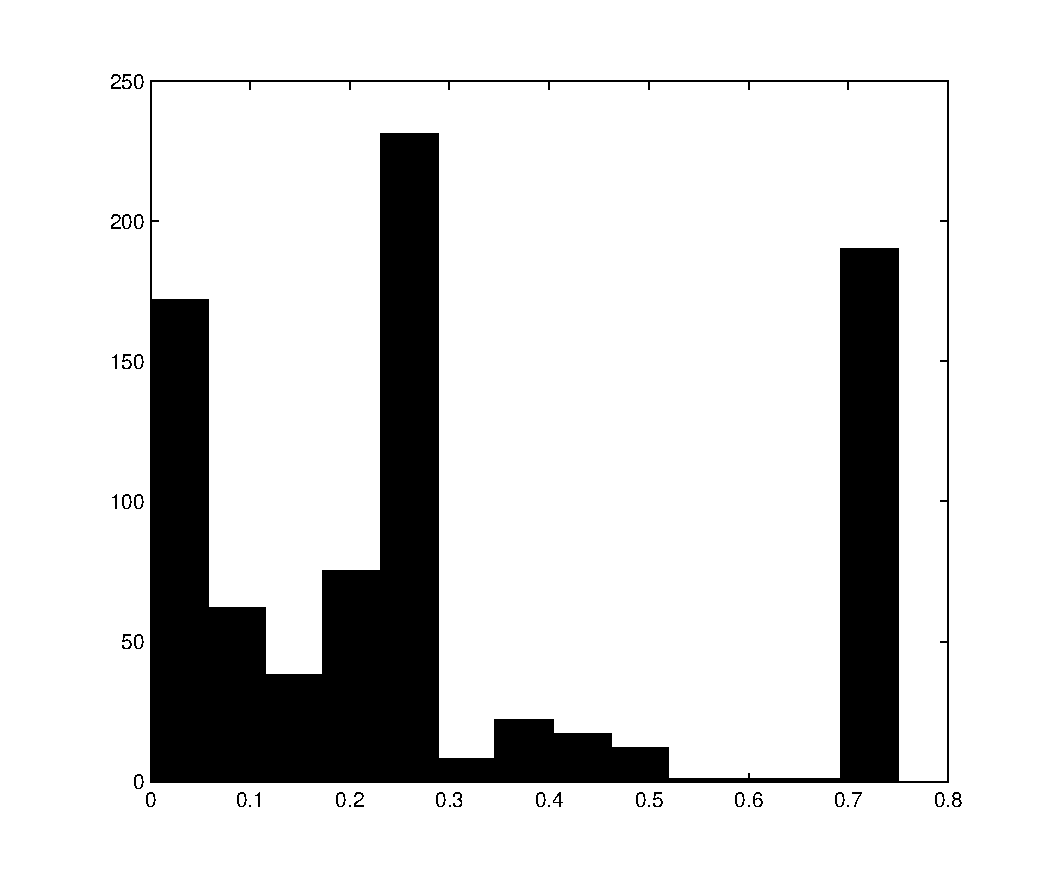
\includegraphics[scale=0.40]{../plots/absolute-deviations.eps}
      \caption{\textbf{TODO}}
      \label{dist-1}
\end{figure}
We see that the distribution is multimodal and discrete. 
Parametric tests such as the z-test and the t-test have been shown to have weaker statistical power in many families of multimodal distributions such as mixtures of Gaussians \cite{???}.
Rank-based tests tend to be more robust to the multimodality and in fact don't depend on the actual values on the relative frequency of the ranks in the test set.



